
\newcommand{\shuki}  {周期}
\newcommand{\server} {巡査}


\section{Introduction}



\subsection{問題設定}
辺の長さが与えられた無向グラフ $G = (V,E)$ の上を
1人または複数の\server が一定の速さで動きながら各点を警備する.
各点 $v_i \in V$ には\shuki $q_i$ と利得 $p_i$ が与えられている.
ある点を警備できているとは,どの連続した2回の訪問も間隔がその点の\shuki 以内であることを言う.
警備している点から得られる利得の合計を最大化するのが目的である.
% 直線や星,木などいくつかのトポロジーについて多項式時間アルゴリズムや困難性を示す.

% 複数の\server による警邏

% サイズ $n$ の重み付き無向グラフ $G = (V,E)$ が与えられ,
% この上を1人または複数人の\server が巡回することで点を訪問する.
% 各点 $v_i$ には\shuki $q_i$ につき1回以上訪問する必要があるという制約のもとで,
% 点を訪問することにより得られる利得 $p_i$ の合計を最大化する点部分集合を求めるのが目的である.

% 1人または複数人の\server により,グラフ上のノードに位置する $n$ 個の点
% $x_i (i = 1,\ldots, n)$ をそれぞれの\shuki $q_i$ 以内に巡回する.
% \server が点 $x_i$ を訪問することにより利得 $p_i$ が得られる.

大きく分けて以下の3つの問題を考える.
\begin{itemize}
	\item
	PLPP(Periodic Latency Problem with Profit) : 
	\server が1人のとき,
	警備できる点部分集合を選び,得られる利得の合計を最大化する問題.
	\item
	MPLPP(Multiple server PLPP) :
	\server が複数人のときのPLPP.
	\item
	PLP(Periodic Latency Problem) : 
	全点を警備できる最小\server 数を求める問題.
	この場合は利得は無関係となる.
\end{itemize}

\server は2人以上同時に1つの点に存在してもよいし,
1つの点は複数人の\server により警備されてもよいとする.
\cite{coene2011charlemagne}

より現実的な設定としては,
\server は点を訪問するときに一定時間そこにとどまる必要がある
とするものが考えられるが(以降この時間を待機時間と呼ぶ),
後で説明するように代わりにグラフを変形することにより待機時間は $0$ である問題に帰着できる.


\subsection{記号の定義}
\begin{itemize}
\item $G = (V,E)$ : 無向グラフ.
\begin{itemize}
	\item $V = \set{ v_1, v_2, \ldots, v_n }$
	\begin{itemize}
		\item $p_i$ : $v_i$ を警備することにより得られる利得.
		$p_i \leq 0$ の点は最初に除外してよいので $p_i > 0$ であるとする.
		\item $q_i$ : \shuki .
		% この時間以内に\server が $v_i$ に帰ってこないと $v_i$ を訪問したことにならない.
		どの連続した2回の点 $v_i$ の訪問も間隔が\shuki $q_i$ 以内であるとき
		この点 $v_i$ を警備していると定義する.
		$q_i \geq 0$.
		\item $w_i$ : $v_i$ を訪問したときにそこにとどまる必要がある時間(service time).
		$w_i \geq 0$.
	\end{itemize}
	\item $E \subseteq V \times V$. 辺 $(v_i, v_j) \in E$ を $e_{ij}$ とも書く.
	\item $d(e)$ : 辺 $e \in E$ の重み(長さ).
	$e = (v_i, v_j)$ に対し $d(v_i,v_j)$ や $d_{i,j}$ のようにも表す.
\end{itemize}


\item servers : $S = \set{ s_1, \ldots, s_m }$
\begin{itemize}
	\item 速度1以下で辺上を動く.
	\item $V_{s_i} \subseteq V$ : \server $s_i$ が警備する点の集合.
	\item $V_S     \subseteq V$ : $\dbigcup_{s_i \in S} V_{s_i}$. 
	\server $s_i \in S$ が警備する点の集合の和集合.
\end{itemize}
\end{itemize}



\subsection{トポロジー}
今回はグラフ $G = (V,E)$ のトポロジーとして
\begin{itemize}
	\item Line    : $E = \setmid{ (v_i, v_{i + 1}) }{ 1 \leq i < n }$
	\item Circle  : $E = \setmid{ (v_i, v_{i + 1}) }{ 1 \leq i < n } \cup \set{(v_n, v_1)}$
	\item Star    : $E = \setmid{ (v_i, 0) }{ 1 \leq i \leq n }$
	 端点の一方が原点であるような Tree.
	\item StarC   : $E = \setmid{ (x_i, 0) }{ 1 \leq i \leq n }$, 
	Star で辺の長さ $d_{i,0}$ が全て等しい場合.
	\item Tree    : $n$ 点からなる木.
	\item General : 一般のグラフ.
\end{itemize}
を考えることにする.
Star はNP困難性を示す際に便利なため導入している.
StarC は Star と違い簡単に解ける場合があるため特別に考えることにする.


% \subsection{解の形式}
% PLPP, MPLPP, PLP に対する解としては
% 各\server の訪問する点の集合を求めればよいこととする.
% これは,



% PLPP, MPLPP, PLP に対する\server 達の動きは,
% 各\server $s_i$ の訪問する点とその時刻の組の系列
% \begin{equation}
% (t_{i_1}, x_{i_1}), (t_{i_2}, x_{i_2}), \ldots
% \end{equation}
% という形式で与えるとする.
% すると,各\server の訪問する点の系列が与えられたときにこれが
% 速さ1以下の\server により巡回可能であるかは,
% 系列中で2つの隣り合う
% $(t_{i_j}, x_{i_j}), (t_{i_{j + 1}}, x_{i_{j + 1}})$
% について

% \begin{equation}
% \frac
% { \abs{ x_{i_j} - x_{i_{j + 1}} } }
% { t_{i_{j + 1}} - t_{i_j} } \leq 1
% \end{equation}
% をチェックすればよく,

% ????


\section{The Results}


\subsection{PLPP, MPLPP, PLP の関係}
PLPPは明らかにMPLPPの特殊ケース($m = 1$)であるのでMPLPPへ帰着可能である.
PLPは,
\server 数は点と同数の$n$人あれば自明に警備できることから,
MPLPPを $m = 1$ から $n$ までの場合について順に解き,初めて全点を警備できたとき
(最大化した利得が $\dsum_{i = 1}^n p_i$ に等しいとき)
の $m$ により求められるので,
PLPはMPLPPへ多項式時間帰着可能である.



\subsection{トポロジー間の関係}
Line, Star は Tree の特殊な場合である.
Line は Circle に帰着可能である
(Circle で $d(v_n,v_1)$ を十分大きくすればこの辺は使う必要が無いので Line の解になる).
今回考えるトポロジーについて複雑性の関係を矢印で示すと図\ref{fig:topology_reduction}
のようになる.

\begin{figure}[H]
	\label{fig:topology_reduction}
	\centering
	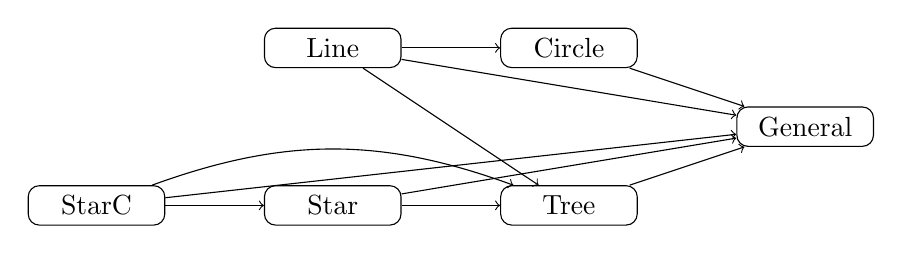
\begin{tikzpicture}
		\tikzset{block/.style={rectangle, text width=1.5cm, text centered, rounded corners, minimum height=0.5cm}};
		\node[draw,block] (Line   ) at ( 0, 0) {Line   };
		\node[draw,block] (StarC  ) at (-3,-2) {StarC  };
		\node[draw,block] (Star   ) at ( 0,-2) {Star   };
		\node[draw,block] (Circle ) at ( 3, 0) {Circle };
		\node[draw,block] (Tree   ) at ( 3,-2) {Tree   };
		\node[draw,block] (General) at ( 6,-1) {General};
		\draw[->] (Line   )--(Circle );
		\draw[->] (Line   )--(Tree   );
		\draw[->] (Line   )--(General);
		\draw[->] (StarC  )--(Star   );
		\draw[->] (StarC  ) to [out=20,in=160] (Tree   );
		\draw[->] (StarC  )--(General);
		\draw[->] (Star   )--(Tree   );
		\draw[->] (Star   )--(General);
		\draw[->] (Circle )--(General);
		\draw[->] (Tree   )--(General);
	\end{tikzpicture}
\end{figure}



以下に現在確かめられている計算複雑性を示す.
太字の部分を証明することにより他の部分を決めることができる.
?の部分はまだ確定していないところである.

\begin{table}[htbp]
	\centering
	\caption{PLPP\label{tab:PLPP}}
	\begin{tabular}{|l|c|c|c|c|c|c|}
	\hline
		& Line & Circle & StarC & Star & Tree & General \\

	\hline
	$q_i = Q$, $p_i = 1$
		& P & P & P & P & P & {\bf NP-hard} \\

	\hline
	$q_i = Q$, arbitrary $p_i$ 
		& P & P & {\bf P} & {\bf NP-hard} & NP-hard & NP-hard \\

	\hline
	arbitrary $q_i$, $p_i = 1$
		& P & P & ? & {\bf NP-hard} & NP-hard & NP-hard \\

	\hline
	arbitrary $q_i$, arbitrary $p_i$ 
		& {\bf P} & {\bf P} & ? & NP-hard & NP-hard & NP-hard \\
	\hline
	\end{tabular}
\end{table}




\begin{table}[htbp]
	\centering
	\caption{PLP\label{tab:PLP}}
	\begin{tabular}{|l|c|c|c|c|c|c|}
	\hline
	 & Line & Circle & StarC & Star & Tree & General \\
	\hline
	$q_i = Q$ & P & ? & P & {\bf NP-hard} & NP-hard & NP-hard \\
	\hline
	arbitrary $q_i$ & ? & ? & ? & NP-hard & NP-hard & NP-hard \\
	\hline
	\end{tabular}
\end{table}




\begin{table}[htbp]
	\centering
	\caption{MPLPP\label{tab:MPLPP}}
	\begin{tabular}{|l|c|c|c|c|c|c|}
	\hline
	 & Line & Circle & StarC & Star & Tree & General \\
	 \hline
	$q_i = Q$,       $p_i = 1$       
		& P & ? & P & NP-hard & NP-hard & NP-hard \\
	\hline
	$q_i = Q$,       arbitrary $p_i$ 
		& {\bf P} & ? & {\bf P} & NP-hard & NP-hard & NP-hard \\
	\hline
	arbitrary $q_i$, $p_i = 1$       
		& ? & ? & ? & NP-hard & NP-hard & NP-hard \\
	\hline
	arbitrary $q_i$, arbitrary $p_i$ 
		& ? & ? & ? & NP-hard & NP-hard & NP-hard \\
	\hline
	\end{tabular}
\end{table}




以下ではまずService Time 無しの場合で考える.
Service Time ありの場合は後述する.




\section{Service Time 無し,\server が1人の場合(PLPP)}


\subsection{PLPP on Line}

Line の場合は実直線上に全ての点を置くことができる.
よって,以降トポロジーが Line の場合については $x$ 軸上に点を置き,
それぞれの座標を $x_1, x_2, \ldots, x_n$ とする.
また,添え字は $x_1 \leq x_2 \leq \cdots \leq x_n$ となっているとしておく.

\begin{theo}
PLPP on Line は多項式時間で解くことができる.
\label{theo:PLPPonLine_1}
\end{theo}

\begin{lemm}
	PLPP on Line に対するある実行可能解 $A$ があったとき,
	$A$ で\server が警備している最も左の($x$ 座標の小さい)点 $v_l$ と
	最も右の点 $v_r$ について,
	区間 $[x_l, x_r]$ を往復する動きにより $A$ と同等以上の利得を得ることができる.
\end{lemm}

\begin{proof}
	$A$ で\server $s$ が警備している点の集合を $V_s$ と書く.
	$x_i < x_j$ であるような任意の $v_i, v_j \in V_s$ について,
	$v_i$ を訪問した後 $v_j$ を訪問し再び $v_i$ に戻るまでの時間について,
	% 時刻 $t_i$ で $x_i$, 時刻 $t_j$ で $x_j$ にいて,
	% その間の時刻 $t_i < t < t_j$ では $x_i$ にも $x_j$ にもいないというような
	% 時刻 $t_i$, $t_j$ が存在する.
	% すると,
	$v_j$ と $v_i$ の間の移動時間の最小値は片道 $x_j - x_i$ なので,
	点 $v_i$ を $q_i$ 以内に訪問できていることから,
	行き帰りの時間について,
	\begin{equation}
		% 2(x_j - x_i) \leq (t_j - t_i) + (x_j - x_i) \leq q_i
		2(x_j - x_i) \leq q_i
	\end{equation}
	が成り立つ.
	同様に点 $v_j$ についても同様に
	\begin{equation}
		2(x_j - x_i) \leq q_j
	\end{equation}
	となる.
	$x_i < x_j$ であるような $v_i, v_j \in V_s $ は任意に選んでいたので
	\begin{equation}
		\sforall v_i, v_j \in V_s . \bigkakko{
			2(x_j - x_i) \leq q_i \text{ and } 2(x_j - x_i) \leq q_j
		}
	\end{equation}
	$x_i$ を基準に考えると
	\begin{equation}
		\sforall v_i \in V_s . \bigkakko{
			\sforall v_j \in V_s . 
			\bigkakko{
				2(x_j - x_i) \leq q_i
			}
		}
	\end{equation}
	すなわち
	\begin{equation}
		\sforall v_i \in V_s . \bigkakko{
			\max_{v_j \in V_s} 2(x_j - x_i) \leq q_i
		}
	\end{equation}
	\server が警備する点のうち左端と右端の点のいずれかが $x_i$ から最も遠い点となるので
	\begin{equation}
		\sforall v_i \in V_s . \bigkakko{
			\max( 2(x_i - x_l), 2(x_r - x_i) ) \leq q_i
		}
		\label{eq:PLPPonLine_2}
	\end{equation}
	ここで,$v_r$ と $v_l$ を往復する動きを考えると,これは式\Ref{eq:PLPPonLine_2}を満たすので
	$V_s$ に含まれる点全てを警備することができる.
\end{proof}

以上により, PLPP on Line では2点間を往復する動きのみ考えれば良いことが分かったので,
${}_n C_2$ 通りの両端を選び,その区間に含まれる点 $x_i$ について
$\max( 2(x_i - x_l), 2(x_r - x_i) ) \leq q_i$ を満たすものを警備するときの利得の合計を
比較することで $O(n^3)$ で最適解を得ることができる.
\qed \Ref{theo:PLPPonLine_1}.

これについてはCoeneら~\cite{coene2011charlemagne}が
$O(n^2)$ で最適解を得るアルゴリズムを与えている.



\subsection{PLPP on Circle}
\begin{theo}
	PLPP on Circle は多項式時間で解くことができる.
	\label{theo:PLPPonCircle_1}
\end{theo}


\begin{lemm}
	PLPP on Circle の最適解は,
	$n$ 本の辺から1本を選び切り開いてできる $n$ 通りの Line での解と,
	\server が Circle 上を周回し続けるときの解を比較することで得られる.
	% (\cite{coene2011charlemagne}に不足していた証明).
\end{lemm}

\begin{proof}
	円周の長さ $d_{1,2} + d_{2,3} + \cdots + d_{n-1,n} + d_{n,1}$ を $L$ とおく.

	ある実行可能解 $A$ があったとき,
	$A$ で警備しているある点 $v_i \in V_s$ について,
	$v_i$ から長さ $L/2$ の位置(円周上でちょうど反対の位置) $\ol{v_i}$ 
	を\server が一度も踏まない場合,
	その点を含む辺を切り開いた Line の解により $A$ を改善することができる.
	どの点 $v_i \in V_s$ についても,円周上でその反対側の位置 $\ol{v_i}$ まで行く場合,
	最後に $v_i$ を出発して $\ol{v_i}$ を訪れ,再び $v_i$ に戻ってくるまでの時間が 
	$q_i$ 以下となるはずである.
	この時間は明らかに $L$ 以上となるので,
	$V_s$ に含まれる全ての点を\shuki $L$ で訪問できる周回運動により少なくとも $A$ 以上の利得を
	得ることができる.
\end{proof}

以上により,最適解は 
$n$ 通りの Line の結果と,周回運動により警備できる点の利得の合計を比較することにより
得られるので,PLPP on Circle は多項式時間で解くことができる.
\qed \Ref{theo:PLPPonCircle_1}.

これについてもCoeneら~\cite{coene2011charlemagne}が
$O(n^2)$ で最適解を得るアルゴリズムを与えている.




\subsection{PLPP on Star}
Star は全ての辺の端点の一方が原点$0$であるグラフである.
Star の場合は $v_i$ と原点の間の辺の長さを $d_{i,0}$ と書く代わりに $d_i$ と書くことにする.

PLPP on Star で $p_i = 1$, $q_i = Q$ の場合は簡単で,
\shuki $Q$ を満たす範囲で原点からの辺の長さ $d_i$ が短い点を順に選んでいけば良い.

一方,$p_i$, $q_i$ のいずれかが任意の場合は NP困難となる.




\begin{theo}
	PLPP on Star with arbitrary $p_i$ は NP困難である.
\end{theo}
\begin{proof}
ナップザック問題からの帰着による.

ナップザック問題とは,入力として
容量 $B$ の容器と,
品物の集合 : $I = \set{ 1, 2, \ldots, n }$ が与えられ,
各品物 $i$ のサイズが $a_i$, 利得が $w_i$ であるとき,
$I$ の部分集合 $I'$ であって
$\dsum_{ i \in I'} a_i \leq B$ を満たしながら
利得の合計 $\dsum_{i \in I'} w_i = W$ となるものが存在するかを判定する問題である.

この問題は PLPP on Star with arbitrary $p_i$ に帰着できる.
各品物 $i$ に対して点 $x_i$ を用意し,
各辺の長さを $d_i = a_i/2$, \shuki を $q_i = B$, 利得を $p_i = w_i$ とする.

すると,ナップザック問題の解 $I'$ が与えられたとき,
$I'$ に対応する点の集合 $V'$ について
\begin{equation}
  \sum_{x_i \in V'} 2 d_i
= \sum_{i \in I'} a_i
\leq B
\end{equation}
より\server は $c'$ の点を全て警備することができ,利得の合計は $W$ となる.
逆に,PLPP on Star の解の点集合 $V'$ が与えられたとき,
利得の合計を $W$ にするような巡回が存在するとき,
$V'$ に対応する品物集合 $I'$ は
\begin{equation}
  \sum_{i \in I'} a_i
= \sum_{x_i \in V'} 2 d_i
\leq B
\end{equation}
を満たすので,ナップザック問題の解とすることができる.
以上によりナップザック問題を帰着できたので
PLPP on Star with arbitrary $p_i$ は NP困難となる.
\end{proof}





\begin{theo}
	PLPP on Star with arbitrary $q_i$ は NP困難である.
\end{theo}
\begin{proof}
3-partition 問題からの帰着による.

3-partition 問題とは,入力として,
容量 $B$ の容器が $k$ 個与えられ,
サイズ $a_i$ が $B/4 < a_i < B/2$ を満たす品物が $3k$ 個与えられるとき,
$k$個の容器に $3k$個の品物を詰めることができるかを判定する問題である.
$B/4 < a_i < B/2$ という制約から品物は3個まで容器に詰めることができるが,
3個ずつ詰められた場合のみ $3k$個の品物を $k$個の容器に詰めることができる.

この問題は PLPP on Star with arbitrary $q_i$ に帰着できる.
点を $3k + 1$ 個用意し,図\ref{fig:star3partitionNPhard}のように
1つの点 $v_0$ は\shuki $q_z = B + 2$, $d_{z0} = 1$, 
その他の点 $v_i$ は\shuki $q_i = k(B + 2)$, $d_{i0} = a_i/2$ というようにする.

\begin{figure}
	\centering
	\caption{3-PartitionのPLPPへの帰着 \label{fig:star3partitionNPhard}}
	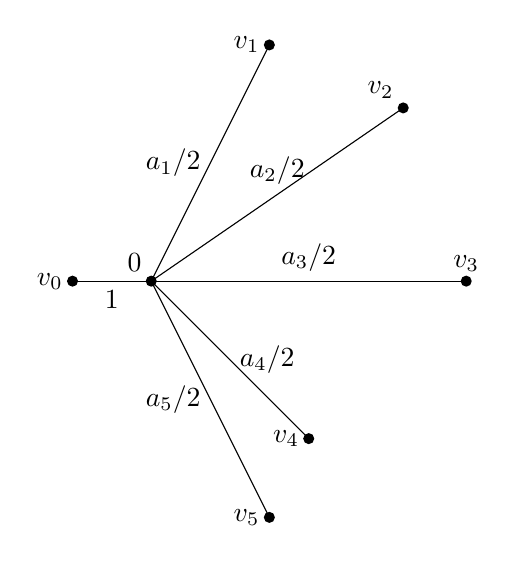
\begin{tikzpicture}
		\fill (-1,0) coordinate (cz) circle (2pt) node [left] {$v_0$};
		\fill ( 0,0) coordinate (O) circle (2pt) node [above left] {$0$};
		\draw[-] (cz) -- node[below] {1} (O);
		\fill ( 1.5, 3  ) coordinate (c1) circle (2pt) node [left] {$v_1$};
		\fill ( 3.2, 2.2) coordinate (c2) circle (2pt) node [above left] {$v_2$};
		\fill ( 4  , 0  ) coordinate (c3) circle (2pt) node [above] {$v_3$};
		\fill ( 2  ,-2  ) coordinate (c4) circle (2pt) node [left] {$v_4$};
		\fill ( 1.5,-3  ) coordinate (c5) circle (2pt) node [left] {$v_5$};
		\draw[-] (O) -- node[left ] {$a_1/2$} (c1);
		\draw[-] (O) -- node[above] {$a_2/2$} (c2);
		\draw[-] (O) -- node[above] {$a_3/2$} (c3);
		\draw[-] (O) -- node[right] {$a_4/2$} (c4);
		\draw[-] (O) -- node[left ] {$a_5/2$} (c5);
	\end{tikzpicture}
\end{figure}

すると,3-partition が可能なときは,
PLPP on Star で $v_0$ からスタートし,
各容器に詰める3個ずつの品物に対応する点を3つ訪問して$v_0$ に戻るという巡回を
することにより,各点の\shuki を満たしながら全点を警備することができる.

逆に,PLPP on Star で全点を警備できるとき,
\server は$v_0$ を訪問した後3つの異なる点を選んで訪問し $v_0$ に戻ってくるということを
$k$ 回繰り返している必要がある.
なぜならば,$v_0$ の\shuki は $B + 2$ なので原点までの行き帰り分の2を引くと
点までの道のりを $B$ まで走ることができるが,$B/4 < a_i$ という条件から高々3つの点しか
訪問することはできず,逆に2つ以下しか訪問せずに $v_0$ に戻るとすると
全点を1周するまでに $k$ 回より多く $v_0$ に戻る必要があり,
各点の\shuki $k(B + 2)$ を満たすことができないからである.
よって,全点を1周できたときには3個ずつの点 $k$ 組に分割できたことになるので
3-partitionの解となる.

以上により3-partition問題を帰着できたので,
PLPP on Star with arbitrary $q_i$ は NP困難となる.
\end{proof}



\subsection{PLPP on Star with $d_i = d$ (StarC)}
以上で表\ref{tab:PLPP}の PLPP on Star の列は決めることができたが,
Starについては $d_i$ が任意ではなく一定とした場合も考えてみる.
この場合は\shuki が定数ならば多項式時間で解くことができる.

\begin{itemize}
\item 
$q_i = Q$ のときは全ての点の訪問のコストが等しいので,
$p_i$ の大きいものから選ぶことで最適解が得られる.
$p_i$ をソートして上位から $\lrfloor{\dfrac{Q}{2d}}$ 個の点を選ぶだけなので,
ヒープソートを用いれば $O\lr{n + \lrfloor{\dfrac{Q}{2d}} \log n}$ の時間で解くことができる.

\item 
$p_i = 1$ のときは $q_i$ の大きいものから選ぶことで,
警備できる点の数を最大化できる.
なぜならば,
警備している点の集合 $V_s$ について,
$x_i \in V_s$ と $x_j \in V \setminus V_s$ であって
$q_i < q_j$ となる組が存在すれば,
辺の長さが全て同じなので $x_i$ を訪問する時間で代わりに $x_j$ を訪問することができ,
$q_i < q_j$ であるからそれ以外の時間は元の\server の動きをそのまま用いることができるためである.
こうして得られる警備する点の集合 $V_s \cup \set{ x_j} \setminus \set{ x_i }$ の利得は
元の利得以上となる.

しかし,$q_i$ の大きいものからいくつ選べるかは自明ではなく,現時点では未解決.

\item 
$p_i$ も $q_i$ も定数でない場合も未解決.
\end{itemize}



\[ \downarrow \textbf{TODO} \downarrow \]
開始時刻指定付き,$q_i$ ちょうどで訪問,$p_i = 1$ という問題を考えると
これは最大独立点集合問題からの帰着によりNP困難であることが示される.

「グラフ $G' = (V',E')$ にサイズ $M$ 以上の独立点集合があるか」
という問題を
「PLPP on StarC, 開始時刻指定付き,$q_i$ ちょうどで訪問,$p_i = 1$ ,
で利得 $M$ 以上の警邏が存在するか」
に帰着する.

$G'$ 上の独立点集合を考えるとき,
$(u_i, u_j) \in E'$ である2点 $u_i, u_j \in V'$ は両方選ぶことはできないが,
これを,PLPP on StarC で訪問されなければならない時刻が重複する時刻があるような
2つの点 $v_i, v_j \in V$ を両方警備することはできないことにより表現する.

$(u_i, u_j) \in E'$ に対しては少なくとも1回
$v_i, v_j$ の両方で同時刻に訪問しなければならないような時刻 $t$ があるようにし,
$(u_i, u_j) \not\in E'$ に対しては
1回もそのような時刻が現れないようにしたい.

各点の指定された訪問時刻の開始時刻を $r_i$ とすると
ある2点 $v_i, v_j$ について
\[
	\sforall k,l \in \Z .
	\lr{ q_i k + r_i \neq q_j l + r_j }
\]
と同値な条件は,ユークリッド互除法により,最大公約数を $gcd(\wc,\wc)$ として
\[
	\Iff 
	\sforall k,l \in \Z .
	\lr { q_i k - q_j l \neq r_j - r_i }
	\Iff
	\sforall n \in \Z .
	\lr{ r_j - r_i \neq gcd(q_i,q_j) \cdot n }
\]
と表される.
同様に,
\[
	\sexists k,l \in \Z .
	\lr{ q_i k + r_i = q_j l + r_j }
	\Iff
	\sexists n \in \Z .
	\lr{ r_j - r_i = gcd(q_i,q_j) \cdot n }
\]

このとき,
$\sforall n \in \Z . \lr{ r_j - r_i \neq gcd(q_i,q_j) \cdot n }$
である2点 $v_i, v_j$ については
$q_i, q_j$ が互いに素でないことが必要になる.




\[ \uparrow  \textbf{TODO} \uparrow \]





\subsection{PLPP on Tree}
PLPP on Star は,PLPP on Tree の特殊な場合なので,
$p_i$, $q_i$ のいずれかが定数でない場合は NP困難となる.
よって,$p_i = 1$, $q_i = Q$ の場合のみを考えるが,
これは Orienteering Problem と呼ばれる問題と同値であり
多項式時間で解くことができることが知られている~\cite{coene2013balancing}.




\subsection{PLPP on General}
一般のグラフについても $p_i = 1$, $q_i = Q$ の場合のみが問題となるが,これはNP困難となる.

\begin{theo}
	PLPP on arbitrary topology with $p_i = 1$, $q_i = Q$ はNP困難である.
\end{theo}
\begin{proof}
ハミルトン閉路問題からの帰着による.

ハミルトン閉路問題とは,入力としてグラフ $G = (V,E)$ が与えられたときに,
全点をちょうど1回訪れる巡回が存在するかを判定する問題である.

これは PLPP の問題に帰着できる.
まずグラフ $G$ を元に完全グラフ $G' = (V,E')$ で,$E'$ の各辺 $e_{ij}$ についてその長さが
\begin{equation}
d_{ij} =
\begin{cases}
	1 & \text{if } e_{ij} \in E \\
	2 & \text{if } e_{ij} \not\in E
\end{cases}
\end{equation}
であるものを考え,
$V$ の点に点を配置し $p_i = 1$, $q_i = |V|$ とする.

すると,PLPP により利得 $|V|$ が得られるかを判定する問題は,
長さ1の辺のみを動いて全点を警備できるかの判定に相当するので,
ハミルトン閉路問題と同値となる.

以上によりハミルトン閉路問題を帰着できたので,
PLPP on arbitrary topology with $p_i = 1$, $q_i = Q$ はNP困難である.
\end{proof}

さらに $d$ をユークリッド距離である場合に制限しても
巡回セールスマン問題からの帰着により NP困難であることが示される.




\section{Service Time 無し,\server が複数人の場合(PLP, MPLPP)}

\server が複数人の場合,どの\server も同じ速さ1以下としているため,
\server がすれ違うような動きはお互いの動きを交換し引き返すような動き方にすることができる.
これにより特に Line の場合,\server は初期配置の $x$ 軸上の順番を保って動くとしてよいことが言える.
ある実行可能解 $A$ についてこのような変換を行ったものを $A^*$ と表すことにする.


\server が複数人の場合,
Star以上に複雑なトポロジーが全てNP困難であることを PLP on Star で示したのち,
残るLine, Circle の場合について調べていく.



\subsection{PLP on Star}
\begin{theo}
	PLP on Star はNP困難である.
\end{theo}
\begin{proof}
Partition からの帰着による.

Partition は,入力としてある非負の値の集合
$X = \set{ a_1, \ldots, a_n }$ が与えられたとき,
これを
\[
	X_1 \cap X_2 = \emptyset,
	\quad
	X_1 \cup X_2 = X,
	\quad
	\sum_{a_i \in X_1} a_i
	 = \sum_{a_i \in X_2} a_i
	 =: k
\]
というように分割できるかを判定する問題である.

これは PLP on Star に帰着できる.
先ほどの Partition の入力に対し,
サイズ $n$ の点の集合 $V = \set{ v_1, \ldots, v_n }$ を考え,
各 $v_i$ について $d_i = a_i / 2$, $q_i = k$ というようにする.
この場合の PLP を解き,\server 数が2人で済むならば
それぞれが\shuki $k$ をちょうど満たしながら独立な点集合を巡回していることになるので,
PartitionはYesとなり,
\server $s_1$, $s_2$ の警備する集合 $V_{s_1}$, $V_{s_2}$ 
がそれぞれ $X$ の分割 $X_1$, $X_2$ となる.
\server 数が3人以上となるならばPartitionはNoとなる.

以上によりPartition問題を帰着できたので
PLP on Star はNP困難である.
\end{proof}



Star の複数人の\server による警邏はNP困難であることが示されたが,
StarC の場合, $\sforall q_i = Q$ の場合は多項式時間で最適解が得られる
ことを示すことができる.


\subsection{MPLPP on StarC, $q_i = Q$}
この場合,点の訪問のコストが全て等しいことから,
利得の大きいものから選べばよいことは明らかであるが,
ちょうど $\lrfloor{\dfrac{mQ}{2d}}$ 点を警備する警邏を以下のように構成できる.

まず,利得の大きいものから $\lrfloor{\dfrac{mQ}{2d}} (=: l)$ 点を求め,
$v_1', v_2', \ldots, v_l'$ とする 
$(p_1' \geq p_2' \geq \cdots \geq p_l')$.

最初に\server $s_1$ が時刻 $t_0$ に原点を出発して
$v_1', v_2', \ldots, v_l'$ を順番に速さ$1$ で動きながら訪問していく.
\server $s_i$ は時刻 $t_0 + (i - 1)Q$ に原点を出発し,
$s_1$ より $(i - 1)Q$ だけ遅れて同じ動きをする.
各\server が原点を出発して $v_1', \ldots, v_l'$ を訪問し
再び原点に戻るまでの時間は $2dl$ であり,
$2dl = 2d \lrfloor{\dfrac{mQ}{2d}} \leq mQ$ であるから,
時刻 $t_0 + (i - 1)Q$ に原点を出発した\server $s_i$ は
時刻 $t_0 + (i - 1)Q + mQ$ までには $v_l'$ まで訪問して原点に戻っており,
時刻 $t_0 + (i - 1)Q + mQ$ に原点を出発して再び同じ動きを繰り返すことができる.

このような動きを繰り返すことで,どの点 $v_i'$ についてもちょうど $Q$ おきに
\server が訪問しているため,$v_1, \ldots, v_l'$ を警備できている.


一方,$m$ 人の\server が警備できる点は高々 $\lrfloor{\dfrac{mQ}{2d}}$ 点である.

任意の長さ $Q$ の時間 $[t_0, t_0 + Q]$ を切り取って考える.
点集合 $V_S \subseteq V$ の点を全て警備しているとき,
$V_S$ の全ての点は少なくとも1回はこの時間に訪問されなければならない.
すると,各点 $v_i \in V_S$ に対して
$[t_0, t_0 + Q]$ のうち少なくとも $2d$ の時間は
$v_i$ に対応する辺 $e_i$ に\server は存在しなければならない($\cdots \star$)
ことを示すことができる.
すると, $m$ 人の\server で $V_S$ の点を訪問するとき
\server が使える時間は明らかに合計 $mQ$ であるので,
$2d \cdot |V_S| \leq mQ$ である必要があり,
これにより $|V_S| \leq \lrfloor{\dfrac{mQ}{2d}}$ が言える.
それでは $\star$ を示す.

任意の点 $v_i \in V_S$ について,
時間 $[t_0, t_0 + Q]$ に少なくとも1回 $v_i$ はいずれかの\server により訪問される.
\begin{itemize}
\item
ある\server が時間 $[t_0 + d, t_0 + Q - d]$ に $v_i$ を
1度でも訪問しているとき(いずれかの\server が $v_i$ に存在する時刻が
$[t_0 + d, t_0 + Q - d]$ の中にあるとき),
少なくともその前後 $2d$ の時間はその\server は辺 $e_i$ 上に存在しなければならず,
またこの時間は $[t_0, t_0 + Q]$ に含まれている.
\item 
$v_i$ が $[t_0 + d, t_0 + Q - d]$ に1度も訪問されないときは,
$[t_0, t_0 + d)$ または $(t_0 + Q - d, t_0 + Q]$ に少なくとも1度訪問される.
$[t_0, t_0 + d)$ に訪問される場合,点 $v_i$ に\server が存在した
最後の時刻を $t_e \in [t_0, t_0 + d)$ とすると,
$t_e + Q$ までに再び $v_i$ は訪問されるはずである.
$[t_e, t_0 + Q - d]$ に再び訪問されることはないときを考えているので,
再度訪問される時刻は $[t_0 + Q - d, t_e + Q]$ に含まれることになる.
すると,\server は $[t_0, t_e + d] \cup [t_e + Q - d, t_0 + Q]$ の間は
辺 $e_i$ に存在することになるので,
$[t_0, t_0 + Q]$ の間に合計で少なくとも
$(t_e + d - t_0) + (t_0 + Q - (t_e + Q - d)) = 2d$ の時間
\server は辺 $e_i$ に存在することになる.
$(t_0 + Q - d, t_0 + Q]$ の場合も対称なので同様に考えればよい.
\end{itemize}
以上により $\star$ が示された.






以上から $\lrfloor{\dfrac{mQ}{2d}}$ 点の警邏が最適解であることが分かる.





次に Line の場合を考える.


\subsection{MPLPP on Line, $q_i = Q$}

\begin{theo}
	\label{theo:MPLPPonLine_1}
	MPLPP on Line with $q_i = Q$ は多項式時間で解くことができる.
\end{theo}



まず次の補題を示す.

\begin{lemm}
	\label{lemm:MPLPPonLine_3}
	ある\server $s$ 1人のみにより警備されている点 $x_i$ が存在するとき,
	$s$ が動ける範囲は $\abs{ x - x_i } \leq q_i / 2$ となる.
\end{lemm}

\begin{proof}[Proof of \Ref{lemm:MPLPPonLine_3}]
	もし $s$ が $\abs{ x_{out} - x_i } > q_i /2$ であるような位置 $x_{out}$ に
	行くことがあるとすると,
	$s$ が最後に $x_i$ を出発してからの時間と,
	次に $x_i$ に戻るまでの時間を合わせた時間 $t$ は
	\begin{equation}
		t > 2 \abs{ x_{out} - x_i} > q_i
	\end{equation}
	となるため,
	$x_i$ は $s$ 以外の\server により訪問されていないので
	$x_i$ を警備できていないことになり矛盾する.
\end{proof}



\begin{lemm}
	\label{lemm:MPLPPonLine_2}
	MPLPP on Line, $q_i = Q$ に対するある実行可能解 $A$ について,
	各\server がそれぞれ独立で両端に点がいるような区間を往復する実行可能解であって
	$A$ 以上の利得を得られるようなものが存在する.
\end{lemm}

\begin{proof}[Proof of \Ref{lemm:MPLPPonLine_2}]
	$A$ で警備する点の集合を
	$V_S = \set{ v_1', v_2', \ldots, v_k' }
	 \quad (  x_1' \leq x_2' \leq \cdots \leq x_k'  )$
	とする.
	$A$ は\server の初期順序を保つ動き $A^*$ に変換してあるとし,
	それらを $x$ 軸上の左側から $s_1, s_2, \ldots, s_m$ とする.
	さらに,全ての\server は区間 $[x_1', x_k']$ を動くように変換できる
	($x < x_1'$ を動くものはその時間 $x_1'$ で待機するようにしても損をしないため.
	$x_k' < x$ を動くものも同様).
	また,全点の\shuki が等しいため,同じ点に存在する複数の点はそれらの合計の利得をもつ
	新たな1つの点にまとめることができる.
	よって以下では $x_1' < x_2' < \cdots < x_k'$ となっているとして進める.

	まず $x_1'$ に注目する.
	いま,\server 順序を保つ $A^*$ に変換しており,
	\server は $x_1'$ より左には進まないように変換しているので,
	$x_1'$ に\server $s_i \neq s_1$ が訪れるときは必ず $s_1$ が $x_1'$ に
	存在することになる.
	よって,$s_1$ 以外の\server は $x_1'$ を訪れずに $x_1' < x$ を
	動くようにしてよい (さらに $x_2' \leq x$ としても同じ利得が得られることが分かる).

	補題\Ref{lemm:MPLPPonLine_3}により $s_1$ の可動範囲は
	$[x_1', x_1' + Q/2]$ となるが,
	$s_1$ はこの区間を往復することによりこの区間に存在する全ての点を警備できる
	(PLPP on Line での証明より)ので,
	この区間 $[x_1', x_1' + Q/2]$ まで入ってくる $s_1$ 以外の\server は
	その時間 $x_1' + Q/2$ で待機するようにしてよい.
	より正確には,
	$V_S$ の点のうち
	$x_a$ を超えない最も左にある点の位置を
	$lm(x_a) := \dmin_{ \setmid{ x_i \in V_S }{ x_a \leq x_i } } x_i$, 
	$x_b$ を超えない最も右にある点の位置を
	$rm(x_a) := \dmin_{ \setmid{ x_i \in V_S }{ x_i \leq x_r } } x_i$, 
	と書くことにすると,
	$s_1$ は区間 $[x_1', rm(x_1' + Q/2)]$ を往復すればよく,
	$s_2, \ldots, s_m$ のうち
	$[x_1', x_1' + Q/2]$ の内部を動いていた\server は
	他の\server の動く範囲に交わらない適当な位置に待機させることで取り除き,
	$[x_1', x_1' + Q/2]$ に入ってくる\server は
	$lm(x_1' + Q/2)$ でその時間待機するようにしてよい.

	このような変換の後,
	$lm(x_1' + Q/2)$ を警備している最も添え字の若い\server を $s_j$ とすると,
	$s_j, s_{j + 1}, \ldots, s_m$ と区間 $[lm(x_1' + Q/2), x_k']$
	に存在する点について, $s_1$ のときと同様の変換をさらに行うことができる.
	これを最後まで繰り返すと,
	全ての\server がそれぞれ両端に点が存在するような
	独立な区間を往復(または停止)するような動きに変換できる.
	この変換で $A$ で警備していた点は全て警備できているので $A$ 以上の利得が得られている.
\end{proof}


以上により,各\server の動きとしては
区間 $[x_i, rm(x_i + Q/2)]$ を往復するもののみを考えれば良いため,
$n$ 個の区間 $[x_i, rm(x_i + Q/2)] \quad (i = 1, 2, \ldots, n)$ から
$m$ 個の重複のない区間を選ぶことで最適解が得られる.

PLPならば全ての点を警備する必要があるので,これらの区間を左から重複のないように貪欲に選んでいけば
\server の動きを決定でき,最小\server 数が得られる.

MPLPPの場合は $n$ 個の区間 $I_i := [x_i, rm(x_i + Q/2)]$ について
その区間に含まれる点から得られる利得の合計 $P_i$ を求めておけば,
重み付き区間の選択問題で区間数 $\leq m$ の制限付きの場合を解くことになる.

まず $x_1, \ldots, x_n$ はソートされていなければソートしておく ($O(n \log n)$).

前半の $P_i$ の求め方だが,これは
$x_1, \ldots, x_n$ と $(x_1 + Q/2), \ldots, (x_n + Q/2)$ を
1つの長さ $2n$ の配列に併合し ($O(n)$), 
この配列を先頭から1つずつ見ていって,
\begin{itemize}
	\item $x_i$ なら $p \gets p + p_i$, 
	\item $x_i + Q/2$ なら $P_i \gets p$; $p \gets p - p_i$
\end{itemize}
という操作をしていくことで計算できる.
$p$ は今見ている長さ $Q/2$ の区間に含まれる点の利得の合計を表す一時変数で,0で初期化する.



後半の,重複のない $m$ 個の区間を選び重みの和を最大化する問題は,
以下の漸化式\Ref{eq:MPLPPonLine_DP}に従う動的計画法で
$m \times n$ の表を左上から計算することにより $O(mn)$ で
最適な区間を選択できる.
$h(j)$ は,区間 $I_j$ より左にある交わらない区間のうち最も右にあるものの添え字を返すもので,
$1 \leq j \leq n$ について $O(n)$ の前計算で得られる.
$OPT(i,j)$ は,区間 $I_1, \ldots, I_j$ から 最大 $i$ 個の区間を選ぶときの
重みの合計の最大値を表す.
$OPT(m,n)$ が求めたい利得の最大値となる.
選ばれた区間も表をトレースバックすることにより再計算できる.

\begin{equation}
	\label{eq:MPLPPonLine_DP}
	OPT(i,j) = 
	\begin{cases}
	0 & \text{ if } i = 0 \\
	\max \Bigkakko{
		0,
		OPT(i,j - 1), 
		P_j + OPT(h(j), i - 1)
	} & \text{ if } i \neq 0
	\end{cases}
\end{equation}

このアルゴリズムの計算量は全体で $O(n \log n + nm)$ である.
\qed \Ref{theo:MPLPPonLine_1}.




\subsection{PLP on Line with arbitrary $q_i$}
次に Line で\shuki が任意の場合を考える.
点の\shuki が全て $Q$ であるときは,\server は各々の区間を独立に往復すればよかったが,
\shuki が任意の場合,
動く範囲に交わりがあり往復でもない動きをするのが最適であるような例が存在する.
図\ref{tikz:multiserver_example}は
\server の軌跡(各時刻 $t$ における\server の位置 $x$ を表す関数 $f : t \mapsto x$ のグラフ)
を横軸を点の位置 $x$, 縦軸を時刻として $t$-$x$ 平面に書いたものであるが,
この例では,左から $q_1 = 10$, $q_2 = 2$, $q_3 = 2$, $q_4 = 10$ である4つの点
が存在するとき,図のような動き方をしなければ3人目の\server が必要になる.

\begin{figure}[H]
	\centering
	\caption{複数人の\server が複雑な動きをする例 \label{tikz:multiserver_example}}
	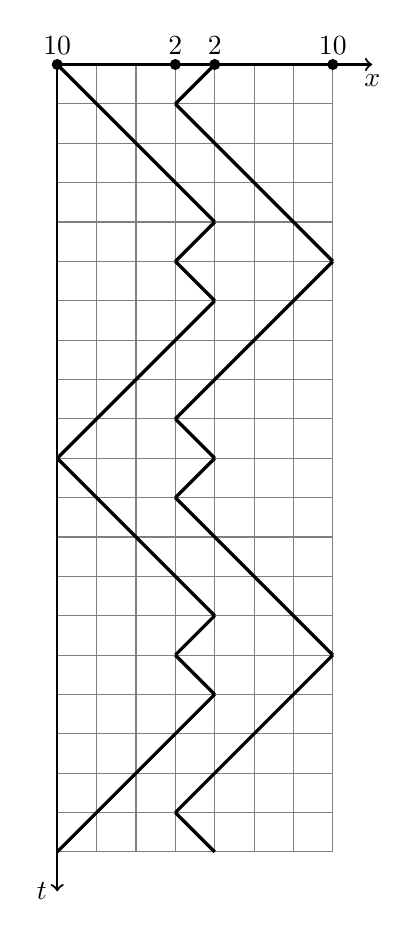
\begin{tikzpicture}
		\draw [help lines,thin,step=5mm] (0,0) grid (3.5,10);
		\draw[thick, ->] (0,10) -- (4,10) node [below] {$x$};
		\draw[thick, ->] (0,10) -- (0,-0.5) node [left] {$t$};

		\fill ( 0  , 10) coordinate (c1) circle (2pt) node [above] {10};
		\fill ( 1.5, 10) coordinate (c2) circle (2pt) node [above] { 2};
		\fill ( 2  , 10) coordinate (c3) circle (2pt) node [above] { 2};
		\fill ( 3.5, 10) coordinate (c4) circle (2pt) node [above] {10};

		\draw[very thick,-] ( 0  ,10  )--( 2  , 8  );
		\draw[very thick,-] ( 2  , 8  )--( 1.5, 7.5);
		\draw[very thick,-] ( 1.5, 7.5)--( 2  , 7  );
		\draw[very thick,-] ( 2  , 7  )--( 0  , 5  );
		\draw[very thick,-] ( 0  , 5  )--( 2  , 3  );
		\draw[very thick,-] ( 2  , 3  )--( 1.5, 2.5);
		\draw[very thick,-] ( 1.5, 2.5)--( 2  , 2  );
		\draw[very thick,-] ( 2  , 2  )--( 0  , 0  );

		\draw[very thick,-] ( 2  ,10  )--( 1.5, 9.5);
		\draw[very thick,-] ( 1.5, 9.5)--( 3.5, 7.5);
		\draw[very thick,-] ( 3.5, 7.5)--( 1.5, 5.5);
		\draw[very thick,-] ( 1.5, 5.5)--( 2  , 5  );
		\draw[very thick,-] ( 2  , 5  )--( 1.5, 4.5);
		\draw[very thick,-] ( 1.5, 4.5)--( 3.5, 2.5);
		\draw[very thick,-] ( 3.5, 2.5)--( 1.5, 0.5);
		\draw[very thick,-] ( 1.5, 0.5)--( 2  , 0  );
	\end{tikzpicture}
\end{figure}


そこでまず,この例から考えられる予想として,
各\server の動きは,最も左を動く $s_1$ から順に
「なるべく右に手伝いに行く」動き方(後で数学的に定義する)により貪欲決定してよいかが気になるが,
実はこれも成り立たない例が存在する.
図\ref{tikz:multiserver_example2}のように,
左から $q_1 = 8$, $q_2 = 2$, $q_3 = 2$, $q_4 = 3$, $q_5 = 6$ である5つの点
が存在するとき,
左図のように $s_1$ がなるべく右に行くような動きをしてしまうと
$x_2,x_3,x_5$ の\shuki を満たす動きが左図のようなものになり,
$x_4$ が\shuki 3以内に訪問されなくなってしまうので3人目の\server が必要になるが,
右図のようにあえて\shuki 6で $x_1$ に戻るような動き方をすれば2人の\server で5つの点を警備できる.



\begin{figure}[H]
	\centering
	\caption{「なるべく右に手伝いに行く」戦略が失敗する例 \label{tikz:multiserver_example2}}
	\begin{tabular}{cc}
	
	\begin{minipage}{0.5\hsize}
		\centering
		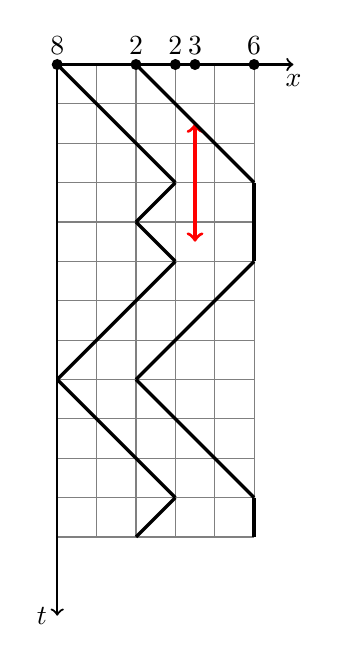
\begin{tikzpicture}
			\draw [help lines,thin,step=5mm] (0,-6) grid (2.5,0);
			\draw[thick, ->] (0,0) -- (3,0) node [below] {$x$};
			\draw[thick, ->] (0,0) -- (0,-7) node [left] {$t$};

			\fill ( 0   , 0) coordinate (c1) circle (2pt) node [above] {8};
			\fill ( 1   , 0) coordinate (c2) circle (2pt) node [above] {2};
			\fill ( 1.5 , 0) coordinate (c3) circle (2pt) node [above] {2};
			\fill ( 1.75, 0) coordinate (c4) circle (2pt) node [above] {3};
			\fill ( 2.5 , 0) coordinate (c5) circle (2pt) node [above] {6};

			\draw[very thick,red,<->] (1.75,-0.75)--(1.75,-2.25);
			\draw[very thick,-] ( 0  , 0  )--( 1.5,-1.5);
			\draw[very thick,-] ( 1.5,-1.5)--( 1  ,-2  );
			\draw[very thick,-] ( 1  ,-2  )--( 1.5,-2.5);
			\draw[very thick,-] ( 1.5,-2.5)--( 0  ,-4  );
			\draw[very thick,-] ( 0  ,-4  )--( 1.5,-5.5);
			\draw[very thick,-] ( 1.5,-5.5)--( 1  ,-6  );
			\draw[very thick,-] ( 1  , 0  )--( 2.5,-1.5);
			\draw[very thick,-] ( 2.5,-1.5)--( 2.5,-2.5);
			\draw[very thick,-] ( 2.5,-2.5)--( 1  ,-4  );
			\draw[very thick,-] ( 1  ,-4  )--( 2.5,-5.5);
			\draw[very thick,-] ( 2.5,-5.5)--( 2.5,-6  );
		\end{tikzpicture}
	\end{minipage}
	
	\begin{minipage}{0.5\hsize}
		\centering
		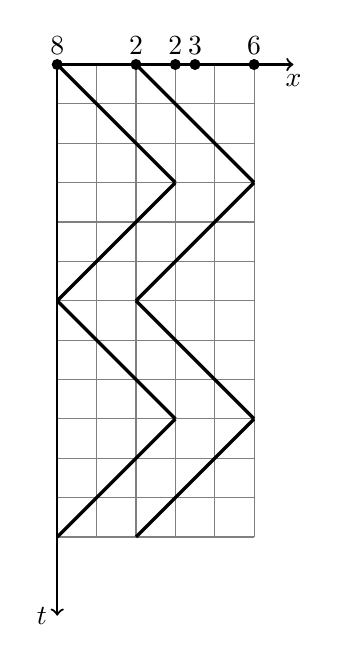
\begin{tikzpicture}
			\draw [help lines,thin,step=5mm] (0,-6) grid (2.5,0);
			\draw[thick, ->] (0,0) -- (3,0) node [below] {$x$};
			\draw[thick, ->] (0,0) -- (0,-7) node [left] {$t$};

			\fill ( 0   , 0) coordinate (c1) circle (2pt) node [above] {8};
			\fill ( 1   , 0) coordinate (c2) circle (2pt) node [above] {2};
			\fill ( 1.5 , 0) coordinate (c3) circle (2pt) node [above] {2};
			\fill ( 1.75, 0) coordinate (c4) circle (2pt) node [above] {3};
			\fill ( 2.5 , 0) coordinate (c5) circle (2pt) node [above] {6};

			\draw[very thick,-] ( 0  , 0  )--( 1.5,-1.5);
			\draw[very thick,-] ( 1.5,-1.5)--( 0  ,-3  );
			\draw[very thick,-] ( 0  ,-3  )--( 1.5,-4.5);
			\draw[very thick,-] ( 1.5,-4.5)--( 0  ,-6  );
			\draw[very thick,-] ( 1  , 0  )--( 2.5,-1.5);
			\draw[very thick,-] ( 2.5,-1.5)--( 1  ,-3  );
			\draw[very thick,-] ( 1  ,-3  )--( 2.5,-4.5);
			\draw[very thick,-] ( 2.5,-4.5)--( 1  ,-6  );
		\end{tikzpicture}
	\end{minipage}
	
	\end{tabular}
\end{figure}


各点の\shuki $q_i$ は,$q_i$ 以内に訪問されていれば良いという条件だったが,
それにより,図\ref{tikz:multiserver_example2}の例ではあえて\shuki 8の点を\shuki 6で訪問
する方が良いために左側から\server の動きを決定できないという難しさが生じてしまった.
% そこで,各点 $x_i$ は $q_i$ ちょうどの時刻は必ず訪問しなければならない
% という制約を設けた場合はどうかを考えてみることにする.
そこでまず,訪問しなければならない時刻に関して最も自由度の少ない,
$t$-$x$ 平面に訪問しなければならない位置と時刻を表す点が全て与えられているときを考えてみることにする.
% 先ほどの\shuki ちょうどで訪問しなければならない問題設定では,各点の訪問すべき点の列同士の
% $t$-$x$ 平面における上下位置には自由度があったが,それもなくして訪問すべき点の列を全て決定
% した場合として考えたものである.
この設定では,左側から\server を割り当て,なるべく右に行く動き方をさせることにより最適解が得られることを
以下のように示すことができる.


\begin{theo}
	\label{theo:xt_decided_1}
	各点 $x_i ( i = 1,2,\ldots,n)$ について,訪問すべき時刻の系列
	$t_{i_1},t_{i_2}, \ldots$ が指定されているとき,
	つまり,$t$-$x$ 平面に\server の動きを書いたときに
	\server が踏むべき点の集合
	$X = \dbigcup_{i = 1}^n \dbigcup_j \set{(t_{i_j}, x_i)}$
	が与えられているとき,
	$s_1$ から順に「なるべく右に行く動き方」で最適解(最小の\server による訪問)を得られる.
\end{theo}



\begin{defi}
	$t$-$x$ 平面において,点 $a = (t_a,x_a)$ に対して
	\begin{alignat*}{3}
	R(a)
	&= R(t_a,x_a)
	&&:= \setmid{(t,x)}{ t < x - x_a + t_a \AND t > -x + x_a + t_a } \\
	L(a)
	&= L(t_a,x_a)
	&&:= \setmid{(t,x)}{ t \geq x - x_a + t_a \OR t \leq -x + x_a + t_a }
	\end{alignat*}
	と定義する.
	$t$-$x$ 平面を全体として,$R(a)$ は $L(a)$ の補集合になる.


\begin{figure}[H]
	\centering
	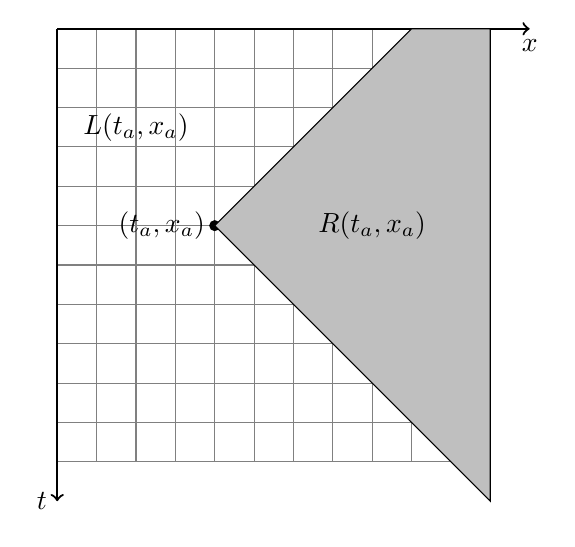
\begin{tikzpicture}
		\draw [help lines,thin,step=5mm] (0,-5.5) grid (5.5,0);
		\draw[thick, ->] (0,0) -- (6,0) node [below] {$x$};
		\draw[thick, ->] (0,0) -- (0,-6) node [left] {$t$};

		\fill ( 2,-2.5) coordinate (ab) circle (2pt) node [left] {$(t_a,x_a)$};

		\filldraw [draw=black, fill=lightgray]
			(ab)--(4.5,0)--(5.5,0)--(5.5,-6)--(ab);

		\node (L) at (1,-1.25) {$L(t_a,x_a)$};
		\node (R) at (4,-2.5) {$R(t_a,x_a)$};
	\end{tikzpicture}
\end{figure}

\end{defi}



\begin{lemm}
	\label{lemm:xt_decided_2}
	\server $s$ の軌跡が $t$-$x$ 平面上のある点 $(t_a,x_a)$ を通るとき,
	$s$ の軌跡は $L(t_a,x_a)$ に含まれる ($R(t_a,x_a)$ を通らない).
\end{lemm}

\begin{proof}[Proof of \Ref{lemm:xt_decided_2}]
	$s$ の軌跡が $(t_a,x_a)$ と $(t_b,x_b) \in R(t_a,x_a)$ を通るとする.
	$(t_1, x_1) \in R$ より
	\begin{equation}
		\label{eq:lemm:xt_decided_2_1}
		t_b < x_b - x_a + t_a
	\end{equation}
	\begin{equation}
		\label{eq:lemm:xt_decided_2_2}
		t_b > -x_b + x_a + t_a
	\end{equation}
	が成り立つ.
	\begin{enumerate}[(i)]
		\item 
		$t_b = t_a$ のときは,式\Ref{eq:lemm:xt_decided_2_1}から $x_b > x_a$ となり,
		$s$ が同時に異なる2点に存在することはできないので矛盾.
		\item $t_b < t_a$ のとき,\server の速さが1以下であることから,
		$s$ が $x = x_b$ から $x = x_a$ に移動するのには少なくとも $\abs{x_b - x_a} = x_b - x_a$ 
		時間かかるので,時刻 $t_b$ 以降で $x_a$ に最初に到達する時刻 $t_a$ は
		$t_a \geq t_b + x_b - x_a$ を満たすが,
		% 一方,時刻 $t_a$ には $x = x_a$ に存在するので
		% $t_a \leq t_a$ より $t_a \geq t_b + x_b - x_a$ となるが,
		これは 式\Ref{eq:lemm:xt_decided_2_2}に矛盾する.
		\item $t_b > t_a$ のときも(ii)と同様.
	\end{enumerate}
	よって, $s$ は $R(a,t_a)$ の点を通ることはできないので,
	$s$ の軌跡は $L(a,t_a)$ に含まれる.
\end{proof}



$t$-$x$ 平面上の点の集合 $X'$ が与えられ,
何人かの\server により $X'$ の点全てを通る必要があるとする.
$X' \neq \emptyset$ ならば,
\server $s$ を1人用意し,$X'$ を担当する\server の中で
最も左を動くようにする.
このとき,次の補題が成り立つ.


\begin{lemm}
	\label{lemm:xt_decided_2_3}
	$s$ の軌跡は $\dbigcap_{a \in X'} L(a)$ に含まれる.
\end{lemm}


\begin{proof}[Proof of \Ref{lemm:xt_decided_2_3}]
	もし $s$ の軌跡が $\dbigcup_{a \in X'} R(a)$ の点 $b = (t_b,x_b)$ を通るとすると,
	ある $a = (t_a,x_a) \in X'$ が存在して $b \in R(a)$ であるが,
	このとき補題\Ref{lemm:xt_decided_2}によると
	$s$ の軌跡は $a$ を通ることができない.
	すると,この $a$ を通る\server $s'$ が新たに必要になるが,
	時刻 $t_a$ において $s$ は $x \geq x_b - \abs{t_b - t_a}$ の領域に存在するため,
	\begin{itemize}
		\item $t_b < t_a$ ならば,
		式\Ref{eq:lemm:xt_decided_2_2}から
		$x \geq x_b - \abs{t_b - t_a} = x_b + t_b - t_a > x_a$.
		\item $t_b = t_a$ ならば,
		式\Ref{eq:lemm:xt_decided_2_1}または\Ref{eq:lemm:xt_decided_2_2}から
		$x \geq x_b > x_a$.
		\item $t_b > t_a$ ならば,
		式\Ref{eq:lemm:xt_decided_2_1}から
		$x \geq x_b - \abs{t_b - t_a} = x_b - t_b + t_a > x_a$.
	\end{itemize}
	より,時刻 $t_b$ において $s'$ は $s$ より左に存在することになる.
	これは $s$ を最も左側にある\server にしたことに矛盾する.
	よって,最も左側の\server $s$ の軌跡は
	$\dbigcup_{a \in X'} R(a)$ の点を含まないので,
	$\dbigcap_{a \in X'} L(a)$ に含まれることが言える.
\end{proof}




\begin{figure}[H]
	\centering
	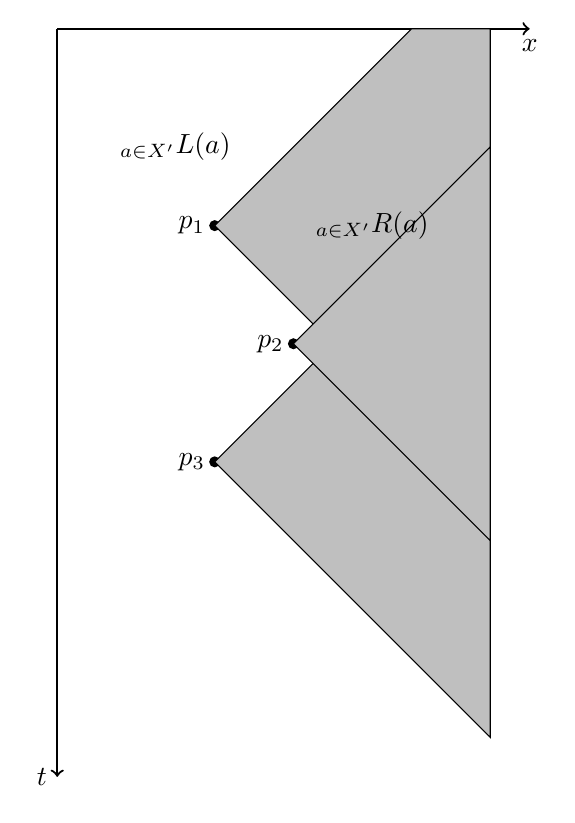
\begin{tikzpicture}
		% \draw [help lines,thin,step=5mm] (0,-8) grid (5.5,0);
		\draw[thick, ->] (0,0) -- (6,0) node [below] {$x$};
		\draw[thick, ->] (0,0) -- (0,-9.5) node [left] {$t$};

		\fill ( 2  ,-2.5) coordinate (p1) circle (2pt) node [left] {$p_1$};
		\fill ( 3  ,-4  ) coordinate (p2) circle (2pt) node [left] {$p_2$};
		\fill ( 2  ,-5.5) coordinate (p3) circle (2pt) node [left] {$p_3$};

		\filldraw [draw=black, fill=lightgray]
			(p1)--(4.5,0)--(5.5,0)--(5.5,-6)--(p1);

		\filldraw [draw=black, fill=lightgray]
			(p3)--(5.5,-2)--(5.5,-9)--(p3);

		\filldraw [draw=black, fill=lightgray]
			(p2)--(5.5,-1.5)--(5.5,-6.5)--(p2);

		\node (L) at (1.5,-1.5) {$\dbigcap_{a \in X'} L(a)$};
		\node (R) at (4,-2.5)   {$\dbigcup_{a \in X'} R(a)$};
	\end{tikzpicture}
\end{figure}



\begin{lemm}
	\label{lemm:xt_decided_3}
	$t$-$x$ 平面上の点の集合 $X'$ に対し,
	$\dbigcap_{a \in X'} L(a)$ の(右の)境界線上にある点の集合を
	\[
		B(X') := \setmid{ b \in X'}{ b \in \bigcap_{a \in X'} L(a) }
	\]
	と表す.
	$X'$ を訪問する\server のうち最も左にあるものを $s$ とすると,
	$s$ はその軌跡が $\dbigcap_{a \in X'} L(a)$ の(右側の)境界と一致する動きが最適であり,
	これにより $B(X')$ の点全体を担当することができる(これを「なるべく右に行く動き」と定義する).
\end{lemm}


\begin{proof}[Proof of \Ref{lemm:xt_decided_3}]
	補題\Ref{lemm:xt_decided_2}より,$s$ の軌跡は
	$\dbigcap_{a \in X'} L(a)$ に含まれるので,
	$s$ が通ることができる点全体は
	$B(X')$ の点の部分集合となる.
	逆に,$s$ は $B(X')$ の点全てを通ることができる.
	なぜならば, $\dbigcap_{a \in X'} L(a)$ の境界線は常に
	傾きが $\pm 1$ であるため,$B(X')$ の点のうち時刻の最も早い点から
	出発して境界線上を動くことにより
	$B(X')$ の点全てを通ることができるためである.

	また,$B(X')$ の点を全て通る動き方は最適である.
	なぜならば,$B(X')$ のうち通らない点がある場合,それらの点の集合を $X''$ と置くと,
	$X'' \cup (X' \setminus B(X'))$ の点全てを通る\server 達の動きは
	そのまま $X' \setminus B(X')$ 全体を通ることができるので,
	$B(X')$ のうち通らない点を残すことにより得をしていないからである.
\end{proof}


以上より,定理\Ref{theo:xt_decided_1}に戻ると,
\[
X_i := 
\begin{cases}
	X & i = 1 \\
	X_{i - 1} \setminus B(X_{i - 1}) & i \geq 2
\end{cases}
\]
として,
$X_i$ が空集合になるまで $i = 1$ から順に $B(X_i)$ を\server  $s_i$ が担当するようにすれば,
% 点全体 $X$ に対して,境界線上の点 $B(X)$ を $s_1$ が担当し,
% $X_2 \neq \emptyset$ ならば
% $B(X_2)$ の点を $s_2$ が担当し,というように
% $X$ を
最適解が得られる.
\qed \Ref{theo:xt_decided_1}.

この定理により得られた結果は
この問題設定に対しては\server を左からなるべく右に行く動き方で割り当てていけば良いということを
数学的に示したものであるが,
有限の手続きにより $X$ 全体を通る\server 数を求めることができるとは限らない.
なぜならば,$X$ の点が時刻$t$に関して周期的になっていない場合 $X$ は $t$ 方向に
無限に長い領域で考える必要があるため $X$ や $B(X)$ が無限集合となるためである.

$X$ が有限集合の場合は $N := |X|$ として
以下の手順により $\Theta(N \log N)$ で
$t$-$x$ 平面上の\server 達の軌跡を描くことができる.

まず,$X$ の各点の元の $t$-$x$ 座標系での表示を
$45^\circ$ 反時計回りに回転した $u$-$y$ 座標系での表示に変換する.
すなわち,各点 $(t_i, x_i)$ を以下のように $(u_i, y_i)$ に変換する.
\[
	\begin{pmatrix}
		u_i \\ y_i
	\end{pmatrix}
	=
	\begin{pmatrix}
		\cos(-45^\circ) & - \sin(-45^\circ) \\
		\sin(-45^\circ) &   \cos(-45^\circ)
	\end{pmatrix}
	\begin{pmatrix}
		t_i \\ x_i
	\end{pmatrix}
	=
	\frc{\sqrt{2}}
	\begin{pmatrix}
		1  & 1 \\
		-1 & 1
	\end{pmatrix}
	\begin{pmatrix}
		t_i \\ x_i
	\end{pmatrix}
\]

次にこの変換後の点 $a_1, \ldots, a_N$ を $u$ の昇順,同着はさらに $y$ の昇順でソートする.
変換・ソート後の点を,
$a_1', a_2', \ldots, a_N'$ とする
 $( u_1 \leq u_2 \leq \cdots \leq u_N)$ .

以降,この $u$-$y$ 平面上の点 $a_1', a_2', \ldots, a_N'$ に対して,
$y$ 軸に平行な scanline を $u = u_1$ の位置から右に動かしていくことを考える.
% $a_1'$ は
% $\sforall a_i' \in \set{a_2', \ldots, a_N'} . \lr a_1' \not\in R(a_i') }$
% を満たすため,必ず最も $x$ 軸方向で左側の\server $s_1$ の担当となる.

\begin{figure}[H]
	\centering
	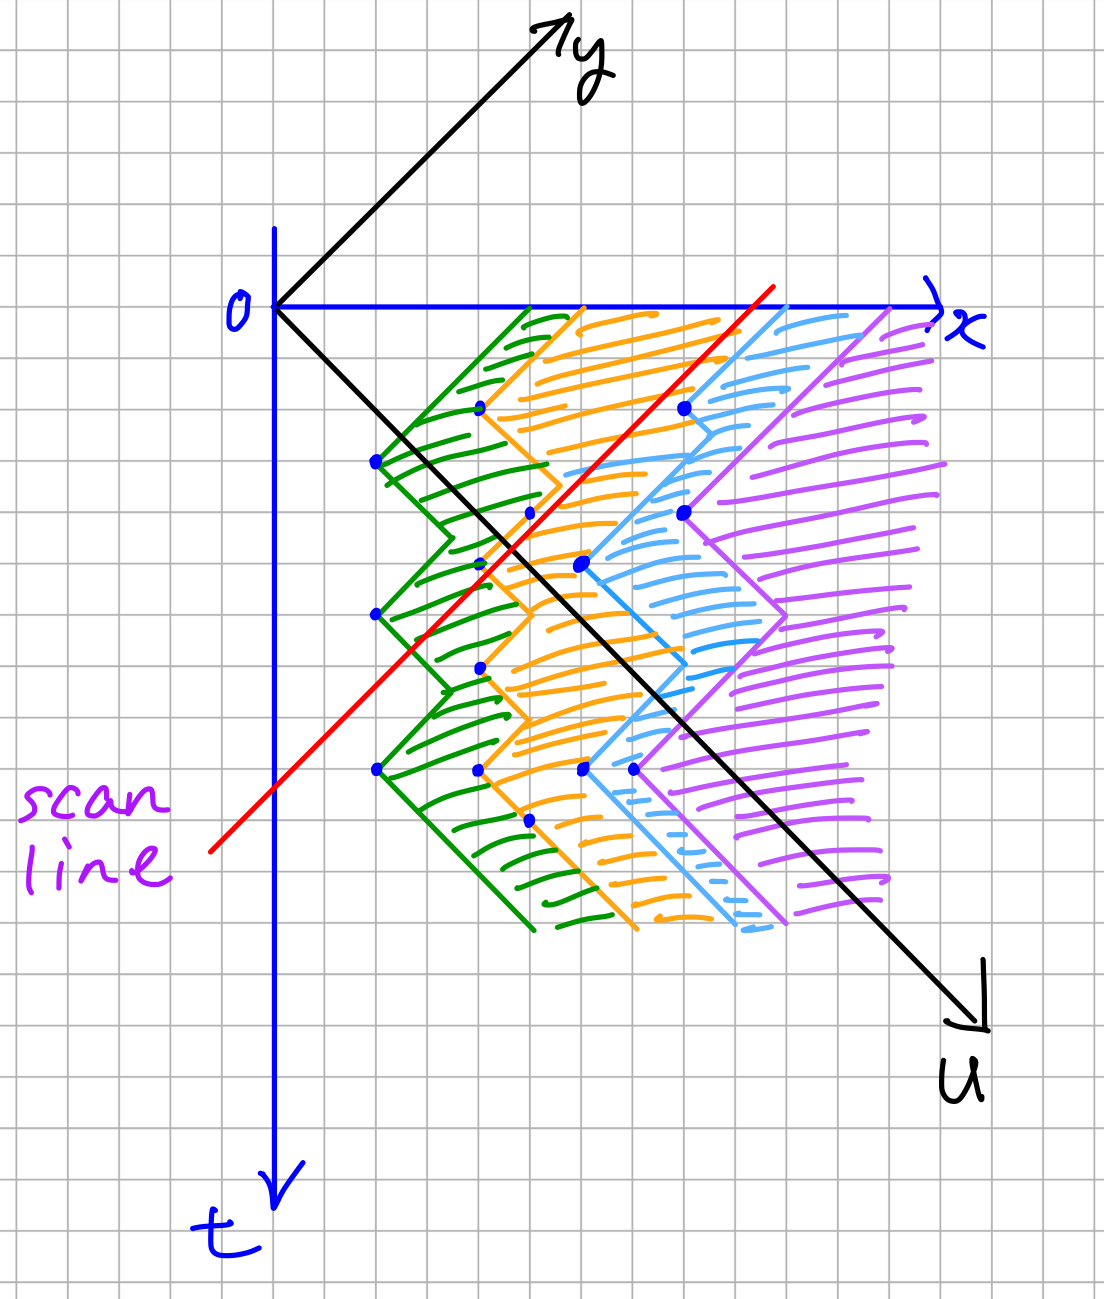
\includegraphics[width=6cm]{./figures/figure2.jpeg}
	\caption{$t$-$x$ 平面上に描いた\server 達の軌跡 \label{fig:uyspace}}
\end{figure}

初めに scanline 全体を色 $c_0$ で塗る.

scanline が $a_1'$ に重なったとき,
scanline の $y > y_1$ の部分を色 $c_1$ で塗る.
次に scanline が $a_2'$ に重なったとき,
$y_2$ が scanline の色 $c_0$ の範囲(境界は含まれる)にあれば
$y_2 \leq y \leq y_1$ と点 $a_2'$ を色 $c_1$ で塗る.
$y_2$ が scanline の色 $c_1$ の範囲にあれば
$y \geq y_2$ と点 $a_2'$ を色 $c_2$ で塗る.


このように,
scanline を動かしていって新たに重なる点 $a_i'$ が scanline の
色 $c_k$ の部分にあれば,$y_i$ 以上の色 $c_{k + 1}$ で塗られた部分に行きつくまで
(無ければ $y = \infty$ まで)色 $c_{k + 1}$ で塗ることを繰り返していく.
このように点と重なるごとに更新されていく scanline の色で $t$-$x$ 平面を塗り分けていくことで
平面上のそれぞれの色 $c_i$ の領域が
$\dbigcup_{a \in B(X_i)} R(a) \setminus \dbigcup_{a \in B(X_{i + 1})} R(a)$
を表すことになり,
その境界線上を各\server が動けばよいことが分かる.

scanline の色として説明した部分は,
scanline の色に対応する区間を管理すればよく,
平衡二分木を用いて,各点と重なる毎に $O(\log N)$ で検索・追加をすれば,
合計 $O(N \log N)$ で平面の塗り分けが完了する.

scanline は各点を通る時点で
各点を担当する\server の番号と軌跡が決められるので,
随時必要な情報を出力していくことができる.

これにより\server の数を知ることができるのも明らかである.




% この過程で各点は scanline と重なった時点で scanline の何色の部分にあるかにより
% それぞれの点を担当する\server の番号が分かり(色 $c_k$ なら\server $s_k$),

% このように scanline を色 $c_1, c_2, \ldots$ で塗っていくと,
% その色の境界が各時点での各\server の軌跡となる.



\section{Service Time 有りの場合}
service time $w_i$ が0でないときは,
元のグラフの点の位置から長さ $w_i / 2$ の枝を生やしてその末端に点を配置し
service time 無しとした問題に帰着できる.
すると,
元の問題で全ての点が原点に集まっている場合($v_1 = v_2 = \cdots = v_n$)でも
帰着後のグラフがStarとなるので,
service time 無しのStarでの結果から任意のトポロジーについて,
PLPPでは $p_i$, $q_i$ いずれかが定数でない場合は NP困難,
PLP, MPLPPでは $p_i = 1, q_i = Q$ でも NP困難となる.

PLPP で $p_i = 1, q_i = Q$ の場合については,
Service time 付き Line は Tree に帰着されるので多項式時間で解ける.
Service time 付き Circle は未解決.
StarC, StarはStar, TreeはTreeに帰着されるので多項式時間で解ける.

% service time が定数の場合($w_i = w$)も考えられる.
% この場合は先ほどNP困難となったもののうち一部は多項式時間で解くことができる.
% (TODO?)


% \subsection{MPLPP}

% \subsubsection{MPLPP on Line with constant frequency}
% MPLPP on Line with constant frequency is $O(n)$-time solvable


\section{TODO}
\begin{itemize}
	\item PLP on Line, ちょうど $q_i$ ごとの時刻は必ず訪問する場合.
% 	\item PLP/MPLPP on Line   with arbitrary frequencies (poly-time?)
	\item PLP/MPLPP on Circle with $q_i = Q$ (poly-time?)
	% \begin{itemize}
	% 	\item 回り続けるか,独立な区間に分けてよいことを示せばよいが
	% 	\item 回り続けるのが最適な例は作れる
	% \end{itemize}
	% \item constant service time の場合をまとめる
% 	\item PLP/MPLPP on Circle with arbitrary frequencies
% 	\item PLPP  on Circle with $p_i = 1, q_i = Q, w_i > 0$
% 	\item PLPP with constant profits, frequencies; boundary between Tree and General
% 	\begin{itemize}
% 		\item Treeはpoly-time
% 		\item GeneralはNP-hard(reduction from Hamiltonian cycle)
% 		\item Treeより複雑だがハミルトン閉路問題を帰着できないようなトポロジー?
% 	\end{itemize}
\end{itemize}

